\documentclass{ximera}

\graphicspath{{./content/02_1_parametric_curves/graphics/}{./graphics/}}

\title{Parametric Curves}
\begin{document}
\begin{abstract}
\end{abstract}
\maketitle


We've dealt with several ways to describe curves in $\mathbb{R}^2$:
\begin{itemize}
\item As the graph of a function. For example, $f(x) = x^2$.
\item As the set of points satisfying an equation. For example, the points $(x,y)$ such that $x^2 + y^2 = 1$.
\item As the set of points satisfying an equation in another coordinate system. For example, $r = \sin(\theta)$ in polar coordinates.
\end{itemize}

Another way that we can describe a curve is using \emph{parametric equations}. When describing a curve using parametric equations, we define $x$ and $y$ in terms of a third variable, often $t$, called the \emph{parameter}. We often think about $t$ as representing time, and imagine the curve being drawn out as $t$ increases. This gives us another way to describe curves in $\mathbb{R}^2$, and potentially describe some new and strange curves.

We can describe the unit circle in $\mathbb{R}^2$ with the parametric equations
\begin{align*}
x & = \cos(t),\\
y & = \sin(t),
\end{align*}
for $0\leq t \leq 2\pi$.

\begin{image}
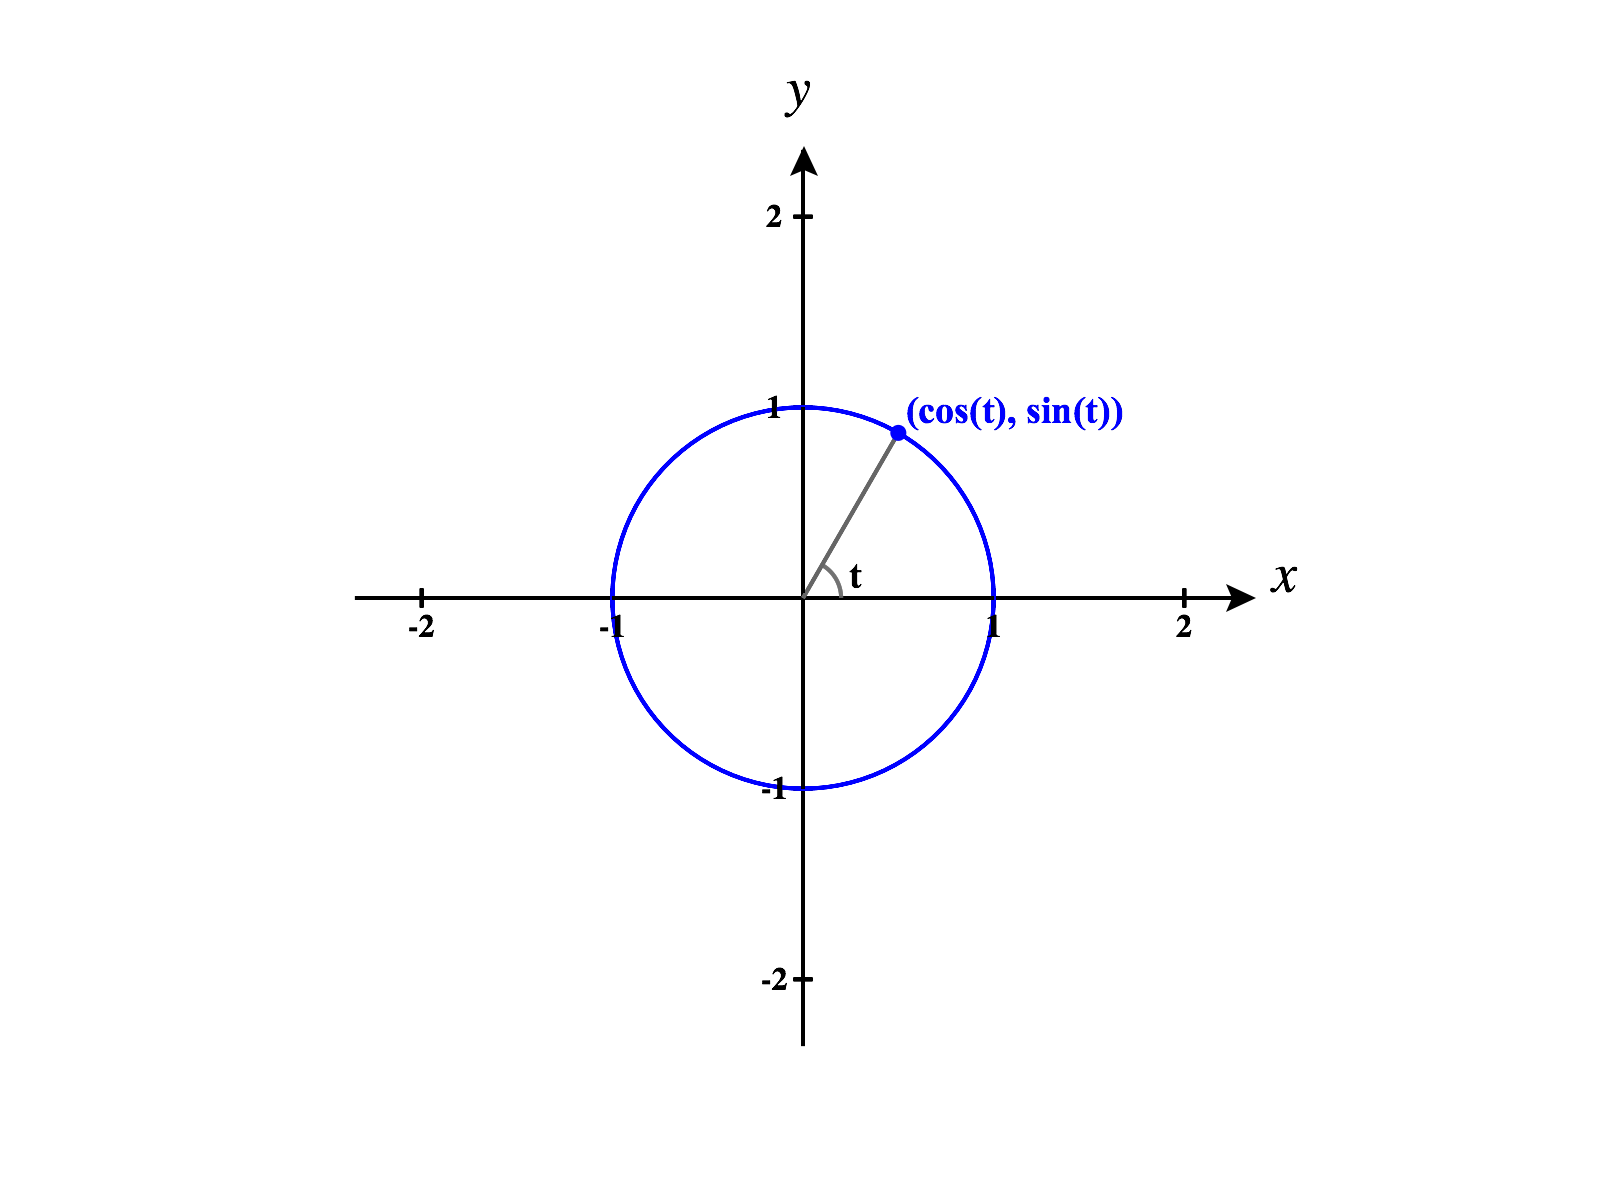
\includegraphics[width = \textwidth]{CalcPlot3D-unit_circle}
\end{image}

We can think of $t$ as giving the angle that a point makes with the positive axis. It can also be helpful to imagine $t$ as representing time, and the parametric equations tracing out the circle as time passes.

\youtube{1J6bT8RE3so}

Consider the parametric equations for the unit circle in $\mathbb{R}^2$:
\begin{align*}
x & = \cos(t),\\
y & = \sin(t),
\end{align*}
for $0\leq t \leq 2\pi$.

We can combine these equations into a single vector,
\[
\vec{x}(t) = (\cos(t), \sin(t))\textrm{ for }0\leq t\leq 2\pi.
\]

We can visualize the vectors $\vec{x}(t)$ tracing out the unit circle as $t$ goes from $0$ to $2\pi$.

\youtube{sYYekBSL4cg}

Notice that we are blurring the distinction between vectors and points. Although we can think of $vec{x}(t)$ as a position vector, we would more commonly think of $\vec{x}(t)$ as a point on a curve. Although this might seem a bit sloppy, it will prove very useful throughout the course. Although intuitively we might prefer to use points, a lot of the computations tools that we'll require are more appropriately used with vectors.

We have defined a function $\vec{x}$ from the interval $[0,2\pi]\subset\mathbb{R}$ to $\mathbb{R}^2$, and this idea provides the motivation behind our definition for paths.

\section*{Parametric Curves in $\mathbb{R}^n$}

\begin{definition}
A \emph{path} in $\mathbb{R}^n$ is a continuous function
\[
\vec{x}:I\subset\mathbb{R}\rightarrow\mathbb{R}^n,
\]
where $I\subset\mathbb{R}$ is an interval.

This is also called a \emph{parametrized curve} or \emph{parametric curve}. When we wish to emphasize that $\vec{x}(t)$ is a vector, we'll call it the \emph{position vector}.
\end{definition}

We'll focus on the cases $n=2$ and $n=3$ in this course.

We defined a path as a continuous function, however, we haven't said what it means for a multivariable function to be continuous. We'll come back to this later, and we'll give a rigorous definition for continuity. For now, this should fit with your intuition: you can draw the path without lifting your pencil from the paper.

Sometimes we care more about the image of a path than how the path is drawn out, and then we refer to a curve.

\begin{definition}
A \emph{curve} $C$ in $\mathbb{R}^n$ is the image of some path $\vec{x}:I\subset\mathbb{R}\rightarrow\mathbb{R}^n$.

In this case, we say that $\vec{x}$ is a \emph{parametrization} for the curve $C$.
\end{definition}

The difference between a curve and a path is largely a matter of perspective: when working with a curve, we pay attention to \emph{what} is drawn; when working with a path, we care about \emph{how} it is drawn.

\begin{example}
There are many different parametrizations for a given curve.

Consider again the unit circle $C$ in $\mathbb{R}^2$. Which of the following are parametrizations for $C$?
\begin{selectAll}
\choice[correct]{$\vec{x}(t) = (\cos(t),\sin(t))$ for $0\leq t\leq 2\pi$}
\choice{$\vec{x}(t) = (\sin(t),\cos(t))$ for $0\leq t\leq \pi$}
\choice{$\vec{x}(t) = (t, \pm \sqrt{1-t^2})$ for $-1\leq t\leq 1$}
\choice[correct]{$\vec{x}(t) = (\sin(2\pi t),\cos(2\pi t))$ for $0\leq t\leq 1$}
\choice[correct]{$\vec{x}(t) = (\cos(t),\sin(t))$ for $-10\leq t\leq 10$}
\end{selectAll}
\end{example}

\begin{example}
In this example, we review a parametrization for the line through points $\vec{a}$ and $\vec{b}$ in $\mathbb{R}^n$.

Given points $\vec{a}$ and $\vec{b}$ in $\mathbb{R}^n$, we obtain a vector starting at $\vec{a}$ and ending at $\vec{b}$ by taking $\vec{b}-\vec{a}$. This vector is parallel to the line through $\vec{a}$ and $\vec{b}$. Then, taking scalar multiples $t(\vec{b} - \vec{a})$ for $t\in\mathbb{R}$, we have a line parallel to the line through $\vec{a}$ and $\vec{b}$. Finally, we add one of the points, $\vec{a}$, to ensure that our line passes through these two points. Thus, we arrive at our parametrization,
\[
\vec{l}(t) = \vec{a} + t(\vec{b}-\vec{a})\textrm{ for }t\in\mathbb{R}.
\]

\begin{image}
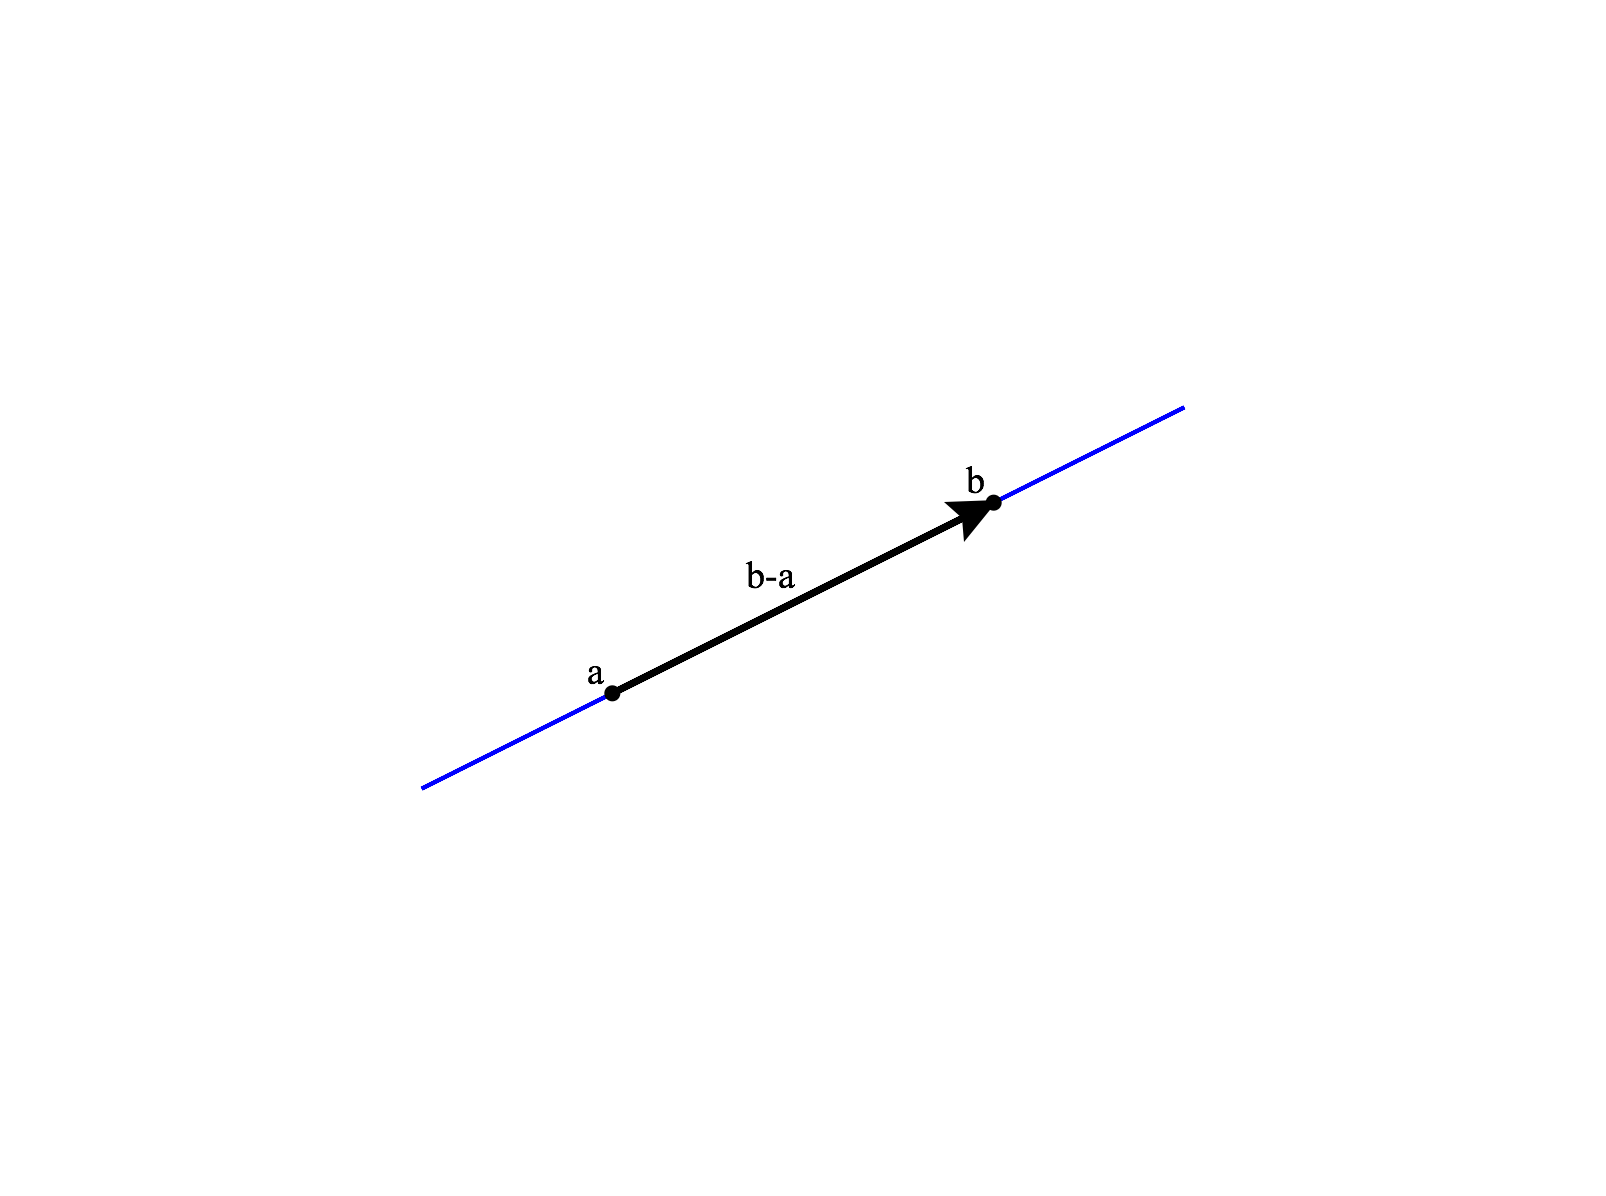
\includegraphics[width=\textwidth]{CalcPlot3D-line_para}
\end{image}
\end{example}

\begin{example}
In this example, we see how we can obtain new transformations from old ones, using linear algebra and simple transformations.

Recall the parametrization for the unit circle in $\mathbb{R}^2$,
\[
\vec{x}(t) = (\cos(t), \sin(t))\textrm{ for }0\leq t\leq 2\pi.
\]

Now, consider the ellipse below.

\begin{image}
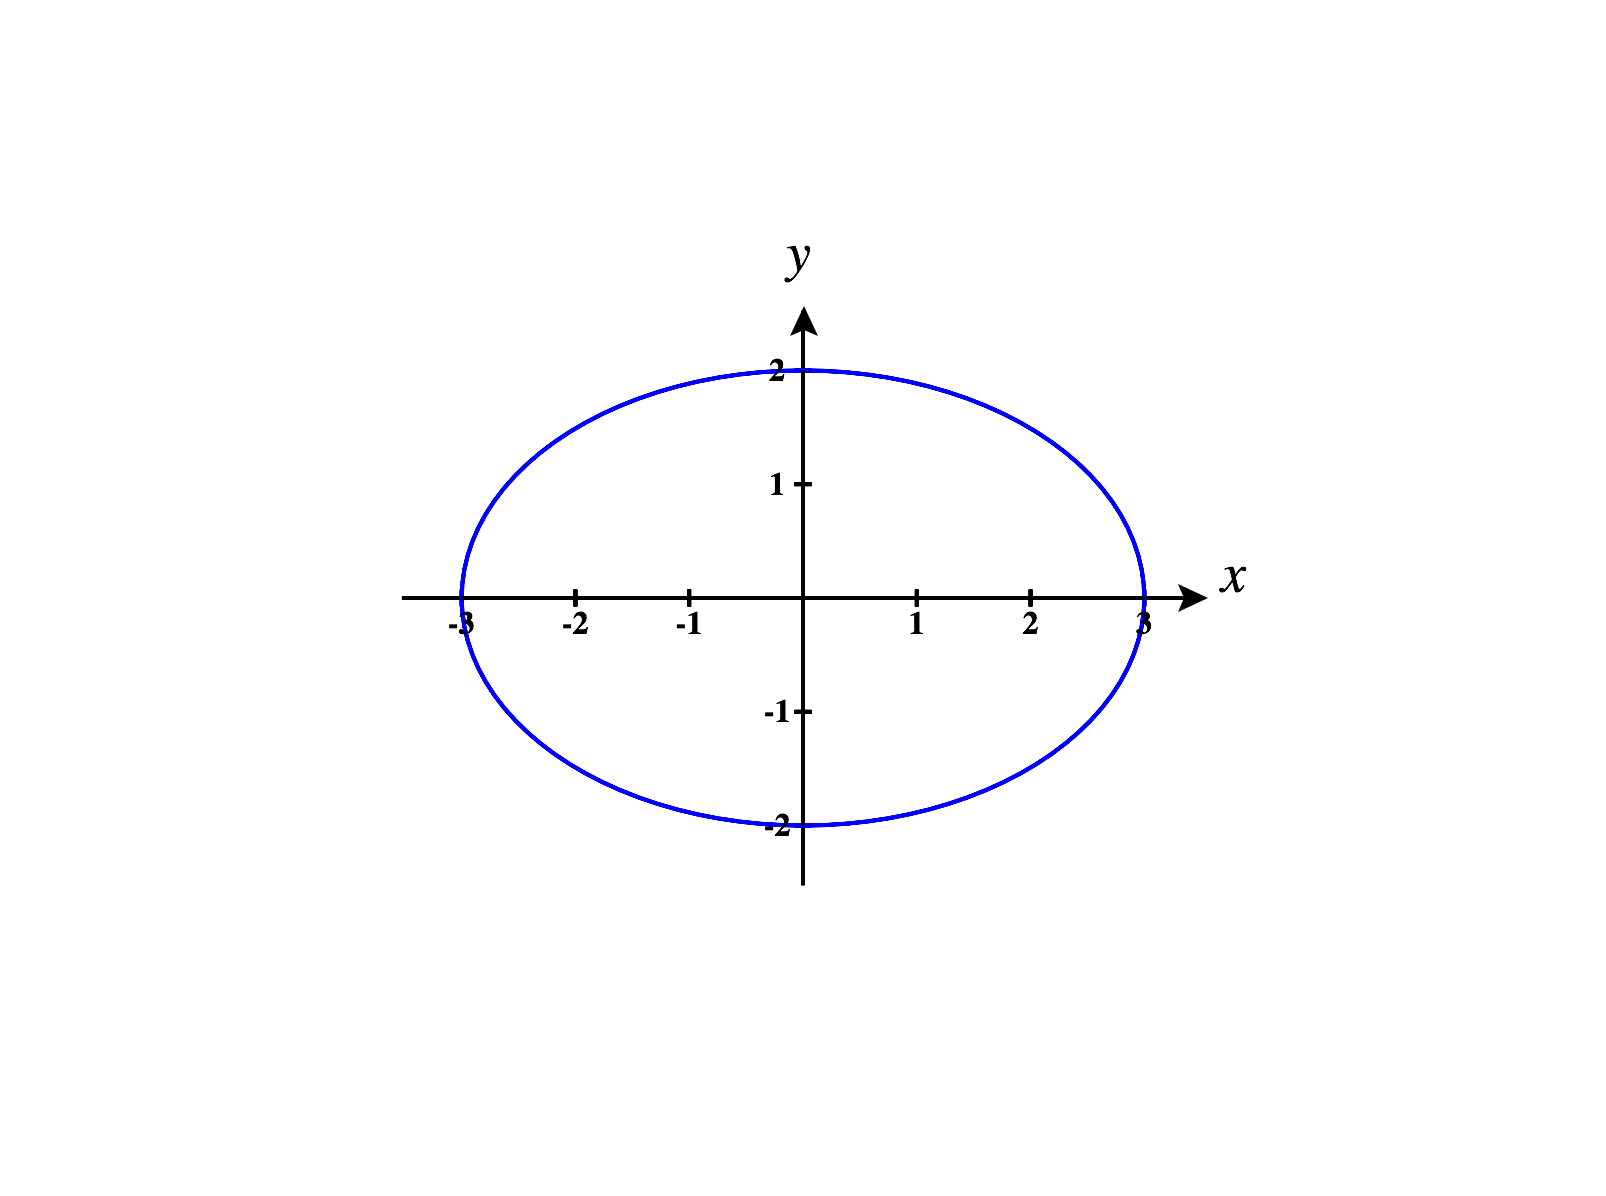
\includegraphics[width=\textwidth]{CalcPlot3D-ellipse}
\end{image}

We can think of this ellipse as the result of stretching the unit circle horizontally by a factor of $3$ and vertically by a factor of $2$. That is, we are applying the linear transformation
\[
\left(\begin{array}{cc}
3 & 0\\
0 & 2
\end{array}\right).
\]
We can apply this to the parametrization for the unit circle, in order to parametrization for the ellipse.
\begin{align*}
\vec(y)(t) &= \left(\begin{array}{cc}
3 & 0\\
0 & 2
\end{array}\right)\left(\begin{array}{c}\cos(t)\\\sin(t)\end{array}\right),\\
&= (3\cos(t), 2\sin(t)).
\end{align*}
Thus, we have a parametrization for the ellipse given by
\[
\vec{y}(t) = (3\cos(t), 2\sin(t))\textrm{ for }0\leq t\leq 2\pi.
\]

Next, consider the following ellipse.

\begin{image}
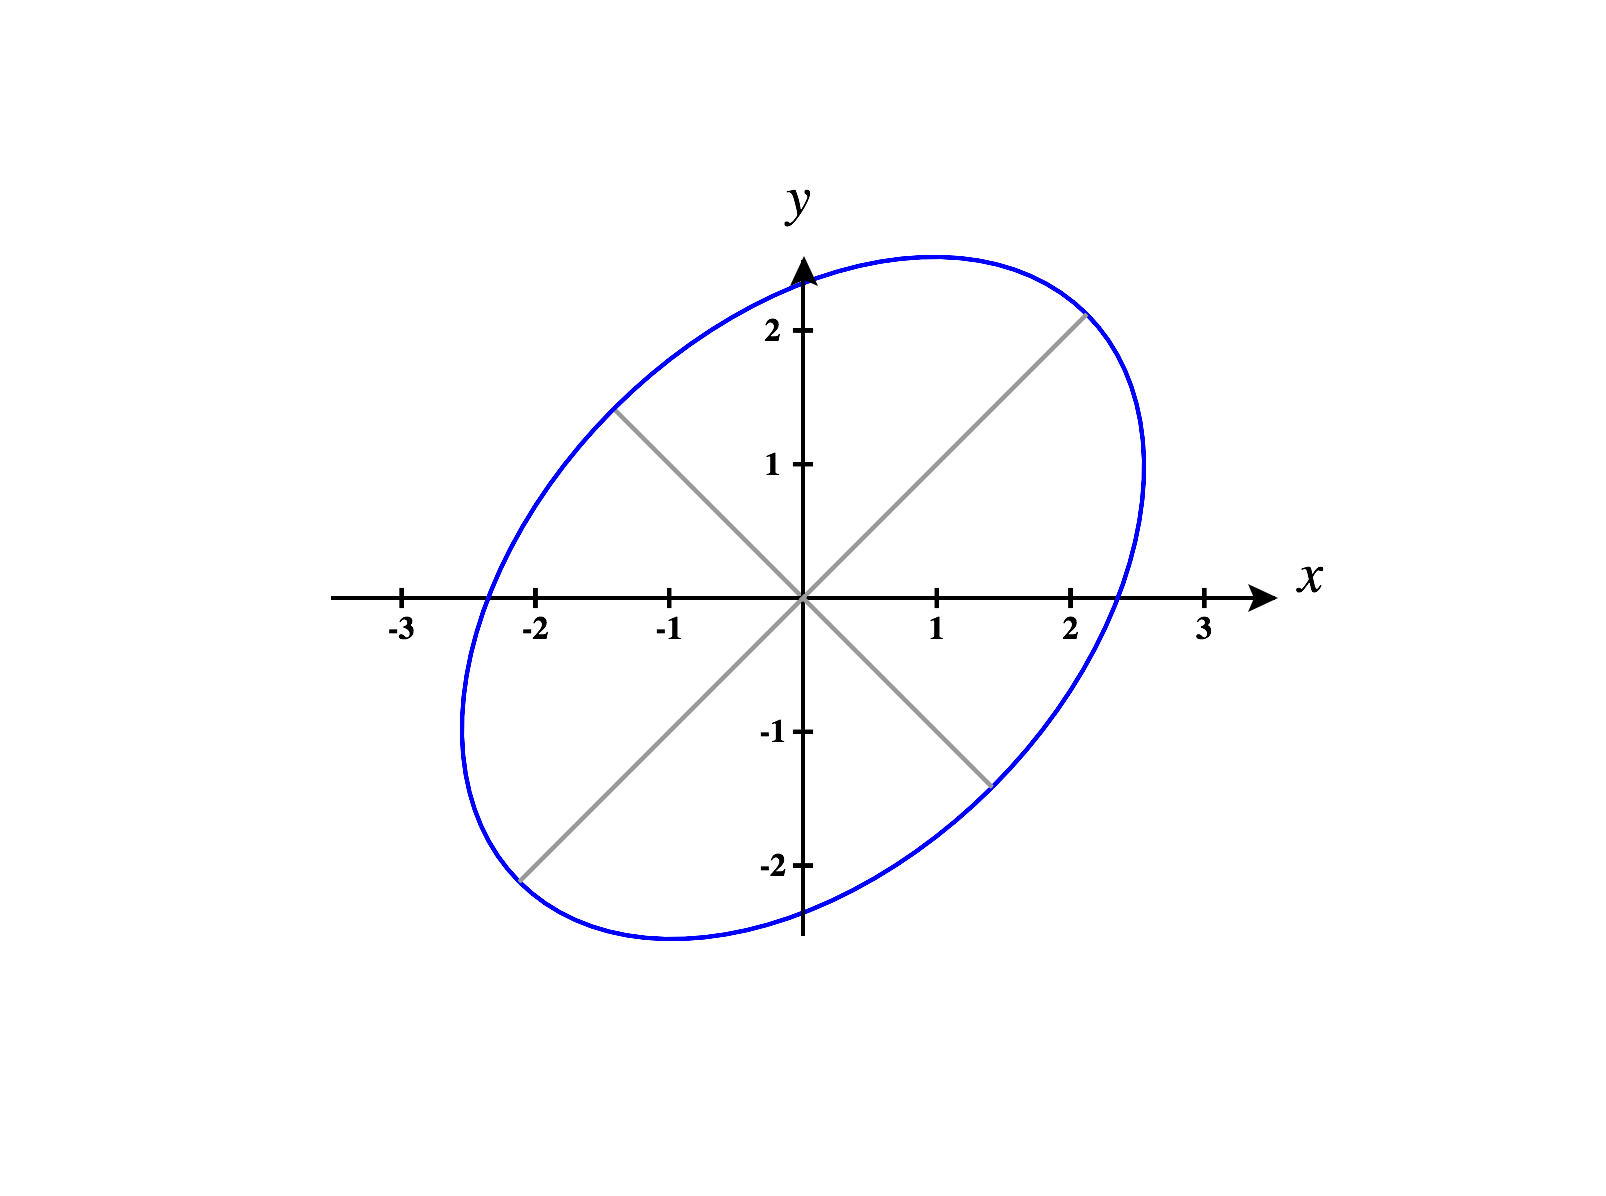
\includegraphics[width=\textwidth]{CalcPlot3D-ellipse_rot}
\end{image}

We can obtain this from our previous ellipse by counterclockwise rotation of $\pi/4$. The matrix for this linear transformation is
\[
\left(\begin{array}{cc}
\cos(\pi/4) & -\sin(\pi/4)\\
\sin(\pi/4) & \cos(\pi/4)
\end{array}\right) = 
\left(\begin{array}{cc}
\answer{1/\sqrt{2}} & \answer{-1/\sqrt{2}}\\
\answer{1/\sqrt{2}} & \answer{1/\sqrt{2}}
\end{array}\right).
\]
Applying this rotation to our parametrization for the previous ellipse, we obtain a parametrization for our new ellipse.
\[
\vec{z}(t) = \answer{(3/\sqrt{2}\cos(t) -2/\sqrt{2}\sin(t), 3/\sqrt{2}\cos(t) + 2/\sqrt{2}\sin(t))}\textrm{ for }0\leq t\leq 2\pi
\]

Finally, we consider an ellipse in $\mathbb{R}^3$, shown below.

\begin{image}
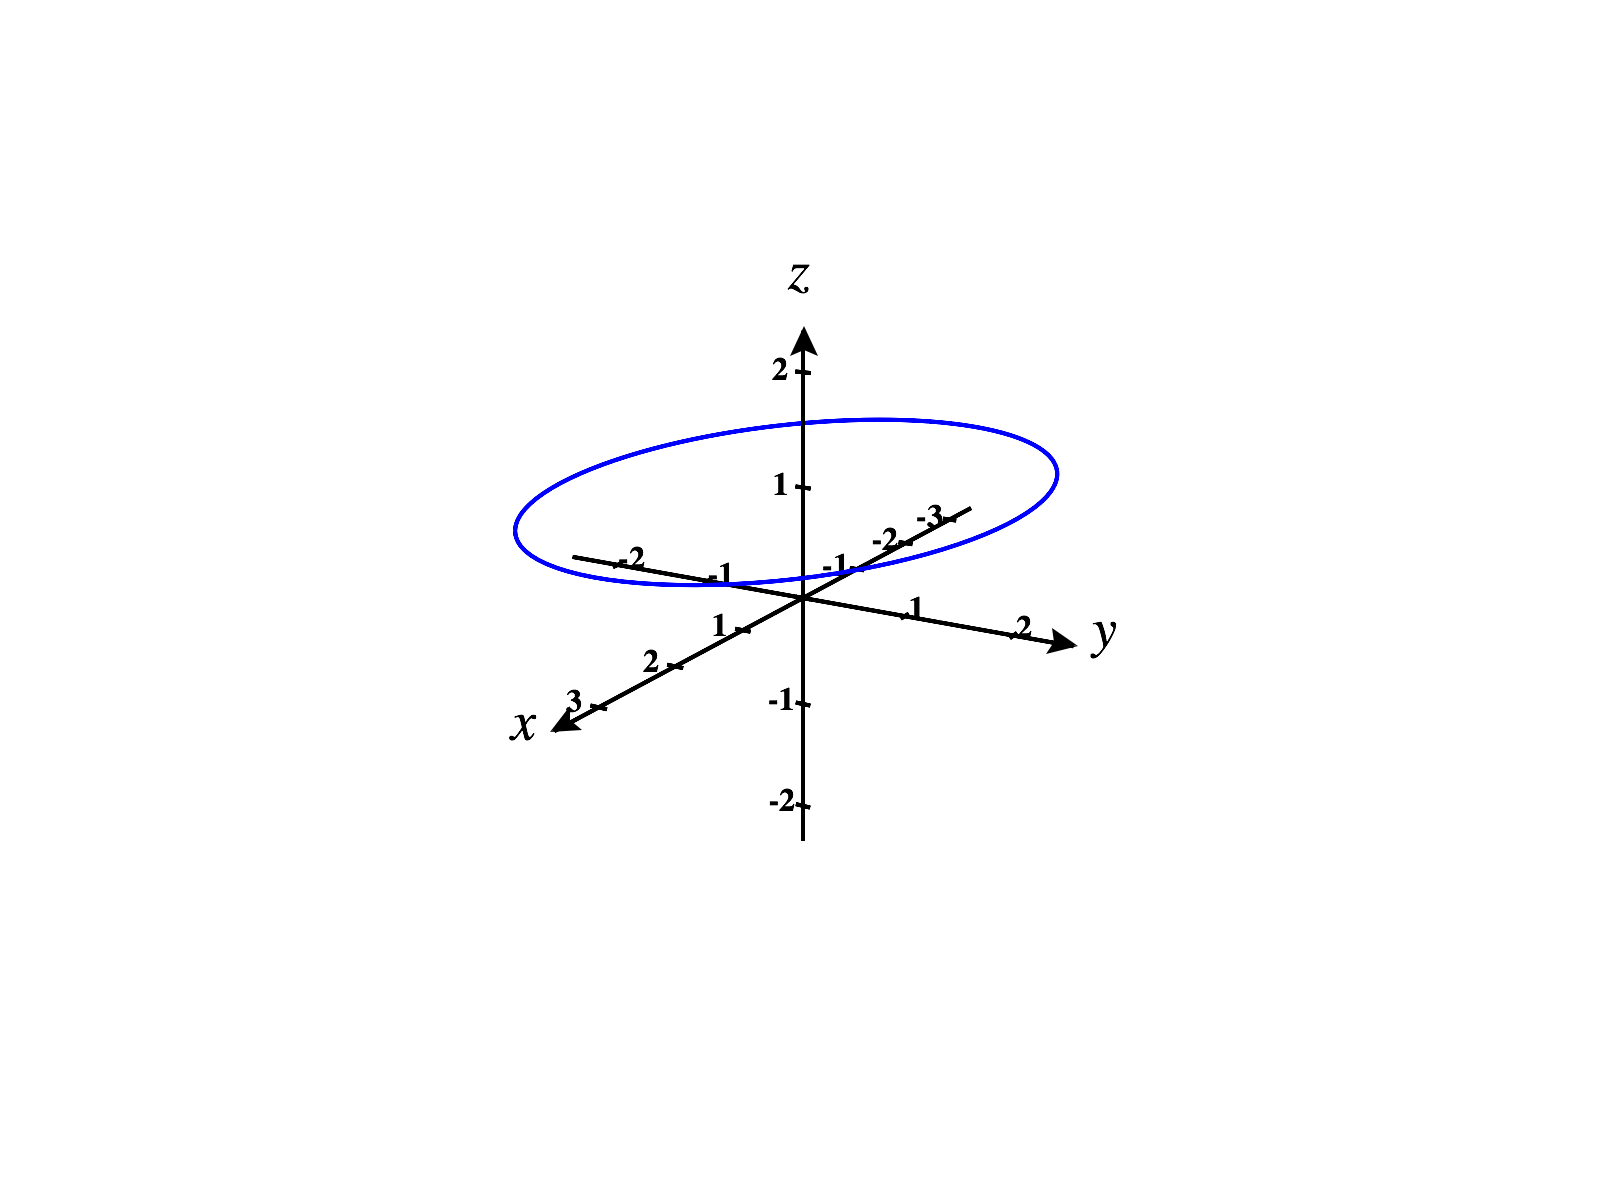
\includegraphics[width=\textwidth]{CalcPlot3D-ellipse_3D}
\end{image}

This ellipse is parallel to the $xy$-plane, and will have constant $z$-coordinate of $1$. Note the similarity to the first ellipse we considered. A parametrization for this ellipse can be obtained by taking the parametrization $\vec{y}$ for our first ellipse in $\mathbb{R}^2$, and appending the constant $z$-coordinate.
\[
\vec{a}(t) = \answer{(3\cos(t), 2\sin(t),1)}\textrm{ for }0\leq t\leq 2\pi
\]
\end{example}

\section*{Examples in $\mathbb{R}^3$}

In this section, we give examples of parametrizations of a couple of more complicated curves in $\mathbb{R}^3$, taking advantage of our previous experience with cylindrical coordinates.

\begin{example}
We'll parametrize the intersection of the cylinder $x^2 + y^2 = 4$ and the plane $z = 7-3x$ in $\mathbb{R}^3$, pictured below.

\begin{image}
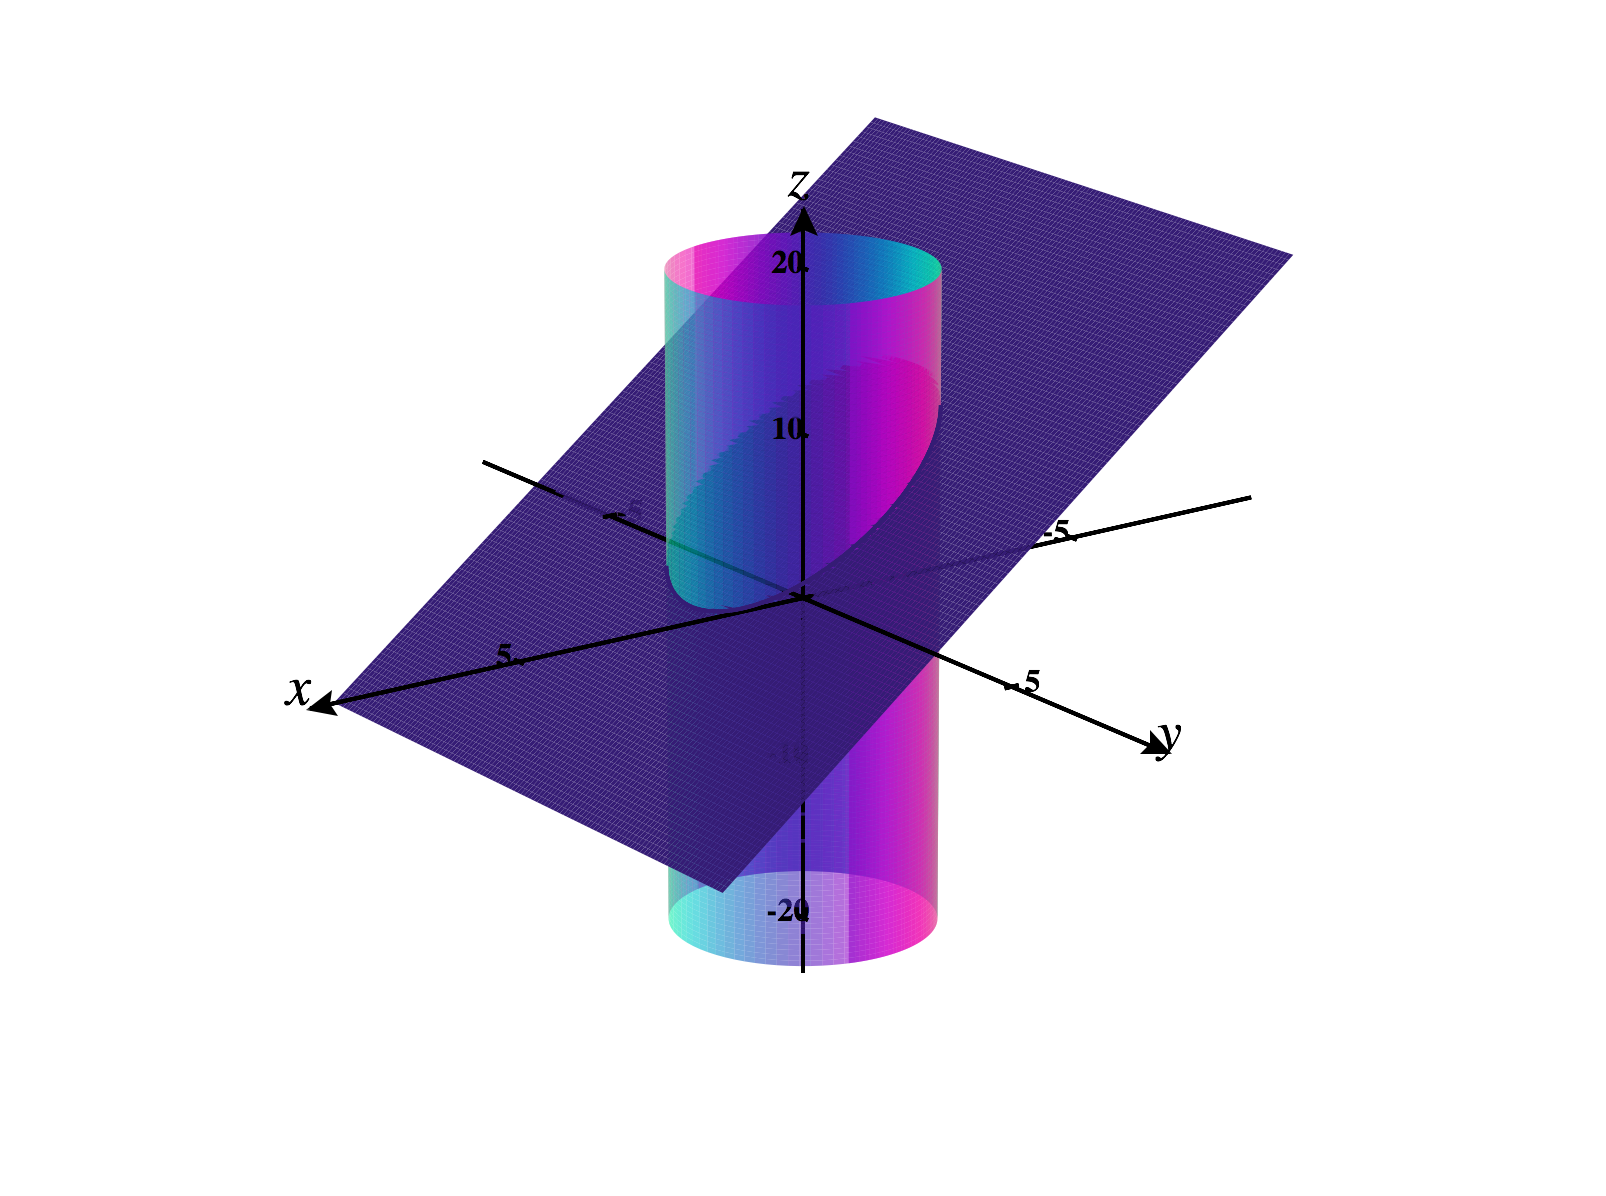
\includegraphics[width=\textwidth]{CalcPlot3D-cyl_plane}
\end{image}

\begin{image}
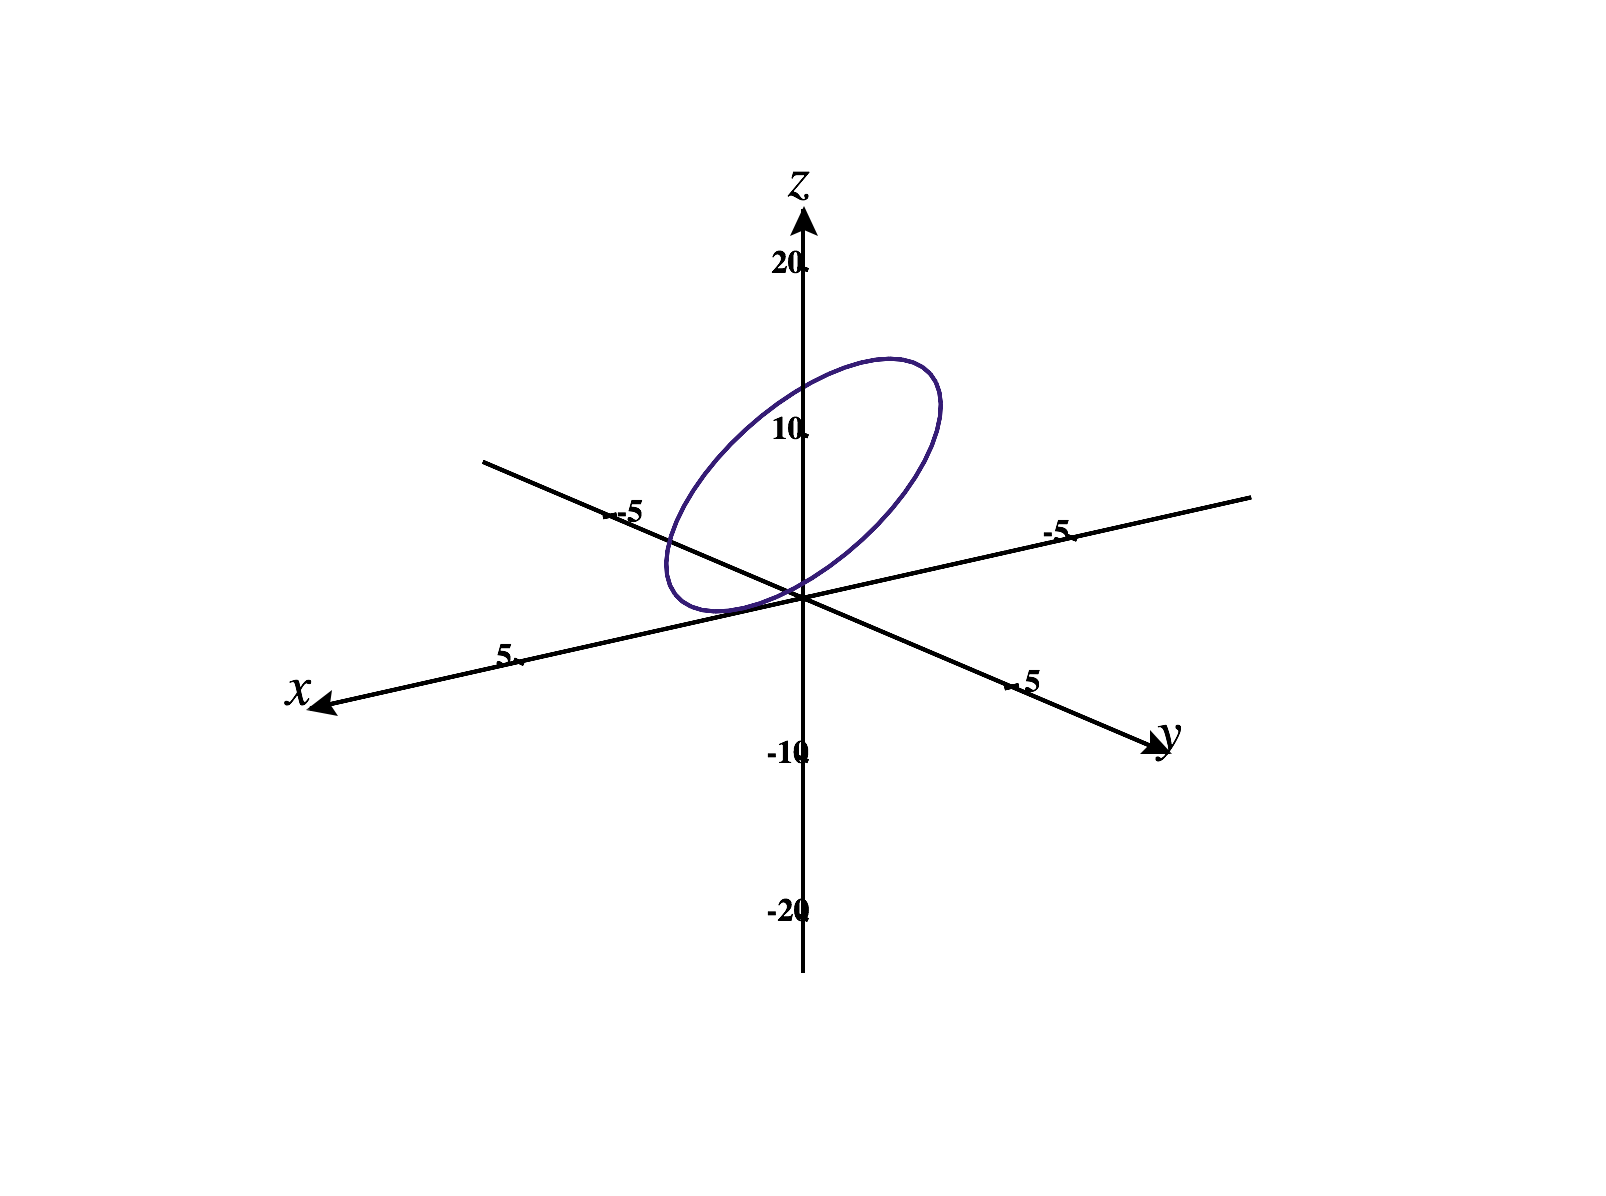
\includegraphics[width=\textwidth]{CalcPlot3D-cyl_plane_curve}
\end{image}


Our $x$ and $y$ coordinates must satisfy $x^2 + y^2 = 4$, which would define a circle, if we were in $\mathbb{R}^2$. Recalling our parametrizations for circles, these coordinates can be written as
\begin{align*}
x(t) &= 2\cos(t)\\
y(t) &= 2\sin(t)
\end{align*}
for $0\leq t\leq 2\pi$.

It remains to write the $z$-coordinate in terms of the parameter $t$. Turning our attention to the equation for the plane, $z = 7-3x$, we have $z$ expressed in terms of $x$. Since we have expressed $x$ in terms of $t$, we can make this substitution to describe $z$ in terms of $t$,
\[
z(t) = \answer{7-6\cos(t)}.
\]

Putting all of this together, we have a parametrization for this intersection given by
\[
\vec{x}(t) = \answer{(2\cos(t),2\sin(t),7-6\cos(t))} \textrm{ for } 0\leq t\leq 2\pi.
\]

\end{example}

\begin{example}
Consider the curve below, which lies on the cone $z^2 = x^2 + y^2$, and makes five rotations around the $z$-axis as the height ranges from $0$ to $1$. We'll refer to this curve as a ``tornado.''

\begin{image}
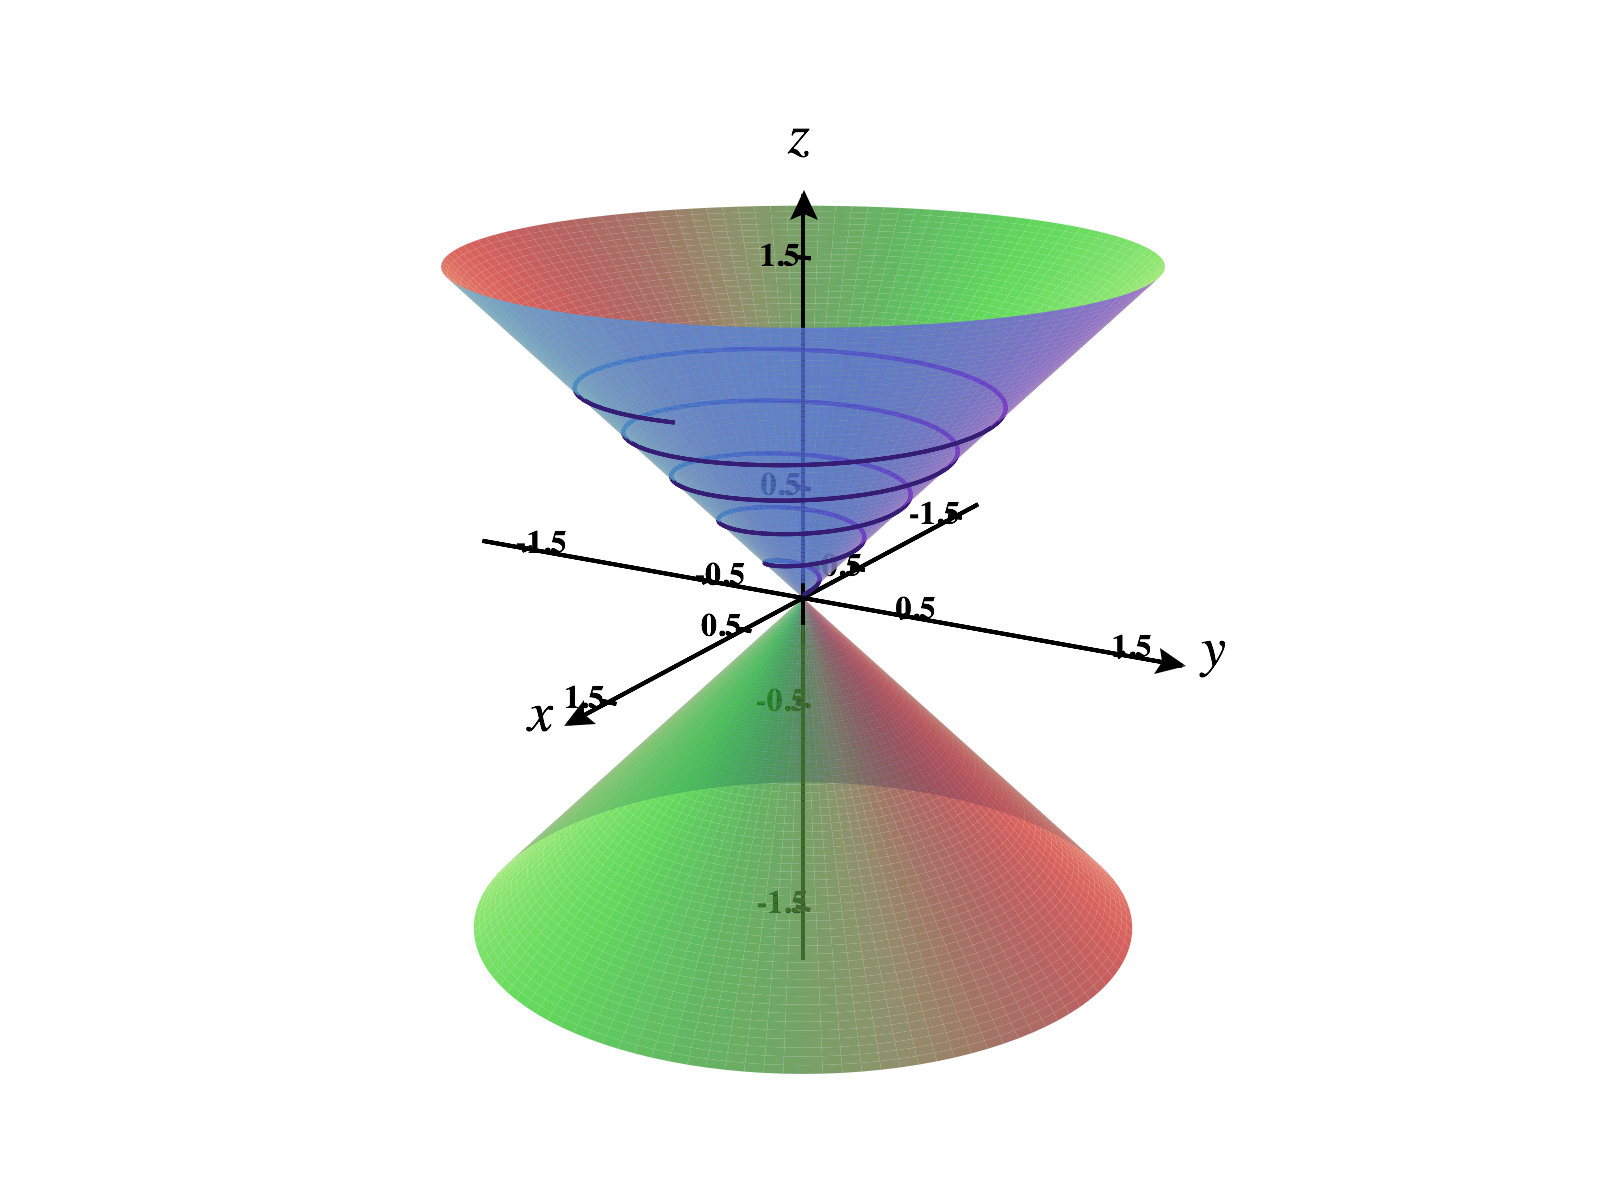
\includegraphics[width=\textwidth]{CalcPlot3D-tornado}
\end{image}

We'll parametrize this curve by thinking about it in cylindrical coordinates, using the height as the parameter.

First, let's consider what's happening with the $z$-coordinate. Since the height of the tornado rangers from $0$ to $1$, so will $z$. We'll set $z = t$, with $0\leq t\leq 1$, and express $x$ and $y$ in terms of $t$ as well.

Now, we turn our attention to the angle $\theta$. As the height ranges from $0$ to $1$, the tornado makes five revolutions, so $\theta$ should range from $0$ to $10\pi$. Thus, expressing $\theta$ in terms of $t$, we let $\theta = 10\pi t$.

Next, we consider the radius $r$. Since we are on the cone $z^2 = x^2 + y^2$, we have $z^2 = r^2$. Since $z\geq 0$, we have $z = r$. Thus, we can write $r$ in terms of $t$ as $r = t$.

Finally, putting all of this together with $x = r\cos\theta$ and $y = r\sin\theta$, we have a parametrization for the tornado given by
\[
\vec{x}(t) = \answer{(t\cos(10\pi t), t\sin(10\pi t), t)} \textrm{ for } t\in [0,1].
\]

\end{example}

\end{document}